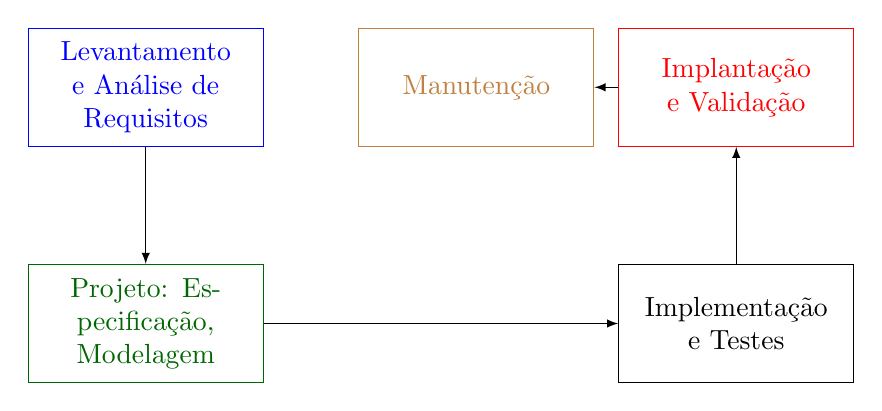
\begin{tikzpicture}
  [cycle/.style={text centered,text width=2.75cm,minimum width=2cm,
    minimum height=1.5cm,draw},every path/.style={->,>=latex,draw}]
  \def\D{2cm}

  \node<1->[cycle,blue] (spec) {Levantamento e Análise de Requisitos};
  \node<2->[cycle,green!40!black] (proj) [below of=spec,yshift=-\D] {Projeto: Especificação, Modelagem};
  \node<3->[cycle] (dev) [right of=proj,xshift=3.25*\D] {Implementação e Testes};
  \node<4->[cycle,red] (deploy) [above of=dev,yshift=\D] {Implantação e Validação};
  \node<5->[cycle,brown] (maintain) [left of=deploy,xshift=-1.15*\D] {Manutenção};
  
  \path<2-> (spec) -- (proj);
  \path<3-> (proj) -- (dev);
  \path<4-> (dev) -- (deploy);
  \path<5-> (deploy) -- (maintain);
\end{tikzpicture}

%%
% Local variables:
% mode: latex
% End:
%%